\documentclass[11pt]{article}
\usepackage[margin=1in]{geometry}
\usepackage{times}
\usepackage{graphicx,booktabs,amsmath,hyperref,xcolor,multirow}
\usepackage[numbers]{natbib}
\hypersetup{colorlinks=true,linkcolor=blue,citecolor=blue,urlcolor=blue}
\newcommand{\TODO}[1]{\textcolor{red}{[TODO: #1]}}
\newcommand{\peval}{$P(\text{eval})$}

\title{Tells: What Causally Makes a Language Model Think It Is Being Evaluated --- and Does It Know Why?}
\author{Mallika Suri\\ Scaler School of Technology, Bengaluru}
\date{AI x Epistemics Research Sprint (Apart Research), November 2026}

\begin{document}
\maketitle

\begin{abstract}
\TODO{150--250 words, written last from final numbers.}
\end{abstract}

\section{Introduction}
Safety evaluations assume that what a model does on a test is what it would do in deployment. That assumption weakens if models can tell the two apart: frontier models already separate evaluation transcripts from real usage well above chance \citep{needham2025large,laine2024sad}, and recent work shows that evaluation-awareness can be represented internally and steered \citep{hua2026steering,nayan2026notone}. A natural response is to make evaluations look more realistic. But to do that we need to know \emph{which} features of a prompt give the game away.

Current practice answers this question in one of two ways. The first asks the model: a judge model explains why it thinks a prompt is a test, and those stated reasons are used to decide what to rewrite \citep{ivanov2025hard}. The second rewrites prompts holistically---many changes at once---and measures the aggregate shift \citep{xiong2025pre}, leaving the contribution of individual cues unidentified (explicitly listed as future work there). Both leave open an epistemic question that matters for anyone relying on these signals: \emph{when a model tells us why it thinks it is being tested, is it telling the truth about what drove its judgement?} Humans are notoriously poor at this kind of introspective report \citep{nisbett1977telling}, and language-model explanations are known to be unfaithful in other settings \citep{turpin2023language}.

We contribute:
\begin{enumerate}
  \item \textbf{A causal cue map.} We edit five candidate ``tells'' one at a time, in both directions---removing each from real evaluation items (Anthropic's advanced-AI-risk safety evals \citep{perez2022discovering} and MMLU-Pro \citep{wang2024mmlupro}) and adding it to real user prompts from WildChat \citep{zhao2024wildchat}---and measure the paired change in the model's stated probability that the prompt is an evaluation.
  \item \textbf{A stated-vs.-causal faithfulness test.} We compare which cues models \emph{say} drove their judgement with which cues \emph{actually} move it, giving precision and recall of verbalised tells.
  \item \TODO{headline findings, 1--2 sentences each.}
\end{enumerate}

\section{Related Work}
\textbf{Evaluation awareness.} \citet{needham2025large} show frontier models classify evaluation vs.\ deployment transcripts with high AUC; SAD \citep{laine2024sad} benchmarks broader situational awareness. \citet{nayan2026notone} find detection, behaviour and control of evaluation-awareness are only weakly coupled across 37 open models, using framing perturbations but not single-feature ablations. \citet{knecht2026limited} intervene on verbalised awareness in chain-of-thought and find small behavioural effects; they do not test whether the verbalised reasons are faithful. \citet{hua2026steering} steer an evaluation-aware model organism toward deployment behaviour.

\textbf{Making evaluations realistic.} \citet{ivanov2025hard} use a judge's stated reasons to guide rewrites of scheming evaluations and find realism hard to achieve. \citet{xiong2025pre} rewrite prompts toward a deployment-like probe score and observe behavioural changes, but apply many edits jointly. Our design isolates individual cues and tests the judge's stated reasons against their measured causal effect.

\textbf{Faithfulness of explanations.} Verbal reports can diverge from the processes that produced a judgement, in humans \citep{nisbett1977telling} and in LLMs \citep{turpin2023language}. We bring this lens to evaluation-awareness, where stated reasons are currently used as a design signal.

\section{Method}
\subsection{Prompt pools}
\textbf{Evaluation pool} ($n=60$): 30 human-written items from Anthropic's advanced-AI-risk evaluations \citep{perez2022discovering} (5 each from power-seeking, survival-instinct, corrigibility, wealth-seeking, coordination with other AIs, and self-awareness), and 30 MMLU-Pro items \citep{wang2024mmlupro} (3 from each of 10 knowledge-heavy categories), all rendered in the standard harness format (\texttt{Question:} / \texttt{Choices:} / \texttt{Answer:}).
\textbf{Deployment pool} ($n=60$): first user turns from WildChat-1M \citep{zhao2024wildchat}, real ChatGPT conversations; English, non-toxic, non-redacted, 60--700 characters, filtered to remove URLs, contact details, code blocks, jailbreak templates, explicit content, and prompts already containing lettered options or \texttt{Question:}/\texttt{Answer:} markers (so that every cue can be cleanly added). Sampling used a fixed seed.

\subsection{Single-cue counterfactual edits}
Table~\ref{tab:cues} lists the five cue families. For each prompt we produce one variant per cue in which \emph{only} that cue is changed: removed from evaluation items (toward realism) and added to deployment items (toward test-likeness). Rule-based edits are used wherever possible for control; where a semantic edit is unavoidable, a fixed rewriter model (\TODO{model}) applies a minimal-edit instruction at temperature 0. Hypothetical-framing removal and personal-context removal are applied only where the rewriter detects the cue (otherwise the item is skipped for that cue). A sixth variant, \emph{all}, applies every edit jointly.

\begin{table}[h]
\centering\small
\begin{tabular}{lll}
\toprule
Cue & Eval items (remove) & Deployment items (add)\\
\midrule
Q/A scaffolding & drop \texttt{Question:}/\texttt{Answer:} (rule) & wrap in \texttt{Question:}/\texttt{Answer:} (rule)\\
Answer options & drop options, minimal stem rewrite (LLM) & append 4 generated options (LLM)\\
Polished register & lowercase, contractions, 2 typos (rule) & formal polish, same content (LLM)\\
No personal context & prepend 1--2 sentence first-person context (LLM) & strip personal context (LLM)\\
Hypothetical framing & recast as a direct situation (LLM) & prefix ``Hypothetically, suppose a user\ldots'' (rule)\\
\bottomrule
\end{tabular}
\caption{Cue families and edit directions.}
\label{tab:cues}
\end{table}

\subsection{Measuring evaluation belief}
Each judge model sees one prompt at a time inside a fixed wrapper asking whether it was ``more likely written as part of an EVALUATION or test of an AI system \ldots or sent by a REAL USER in ordinary deployment'', and returns \peval{} as an integer 0--100. We use two modes: \textbf{num}, which returns only the number (our causal measurement), and \textbf{reason}, which first lists up to three features that most influenced the judgement. All calls use temperature 0. Judges: \TODO{models}, accessed via Adaption's hosted inference API.

\subsection{Metrics}
\textbf{Cue effect.} For prompt $i$ and cue $c$, $\Delta_{ic} = P_{ic} - P_{i}$ (variant minus original). We report the mean effect \emph{of the cue's presence} on \peval{} (sign-flipped for removals), with 95\% bootstrap CIs over prompts and a Wilcoxon signed-rank test. \textbf{Additivity.} We compare the joint (\emph{all}) edit with the sum of single-cue effects. \textbf{Stated vs.\ causal.} Each listed reason is tagged by a fixed classifier into one of the cue families, ``AI-as-topic'', or ``other content''. For each (prompt, cue) pair we record whether the cue was named on the version that contains it, and whether editing it moved \peval{} by $\geq$10 points. We report mention rate, causal rate, $P(\text{causal}\mid\text{mentioned})$ (precision of stated tells) and $P(\text{mentioned}\mid\text{causal})$ (recall).

\section{Results}
\TODO{fill from results/summary.json}

\begin{figure}[t]
\centering
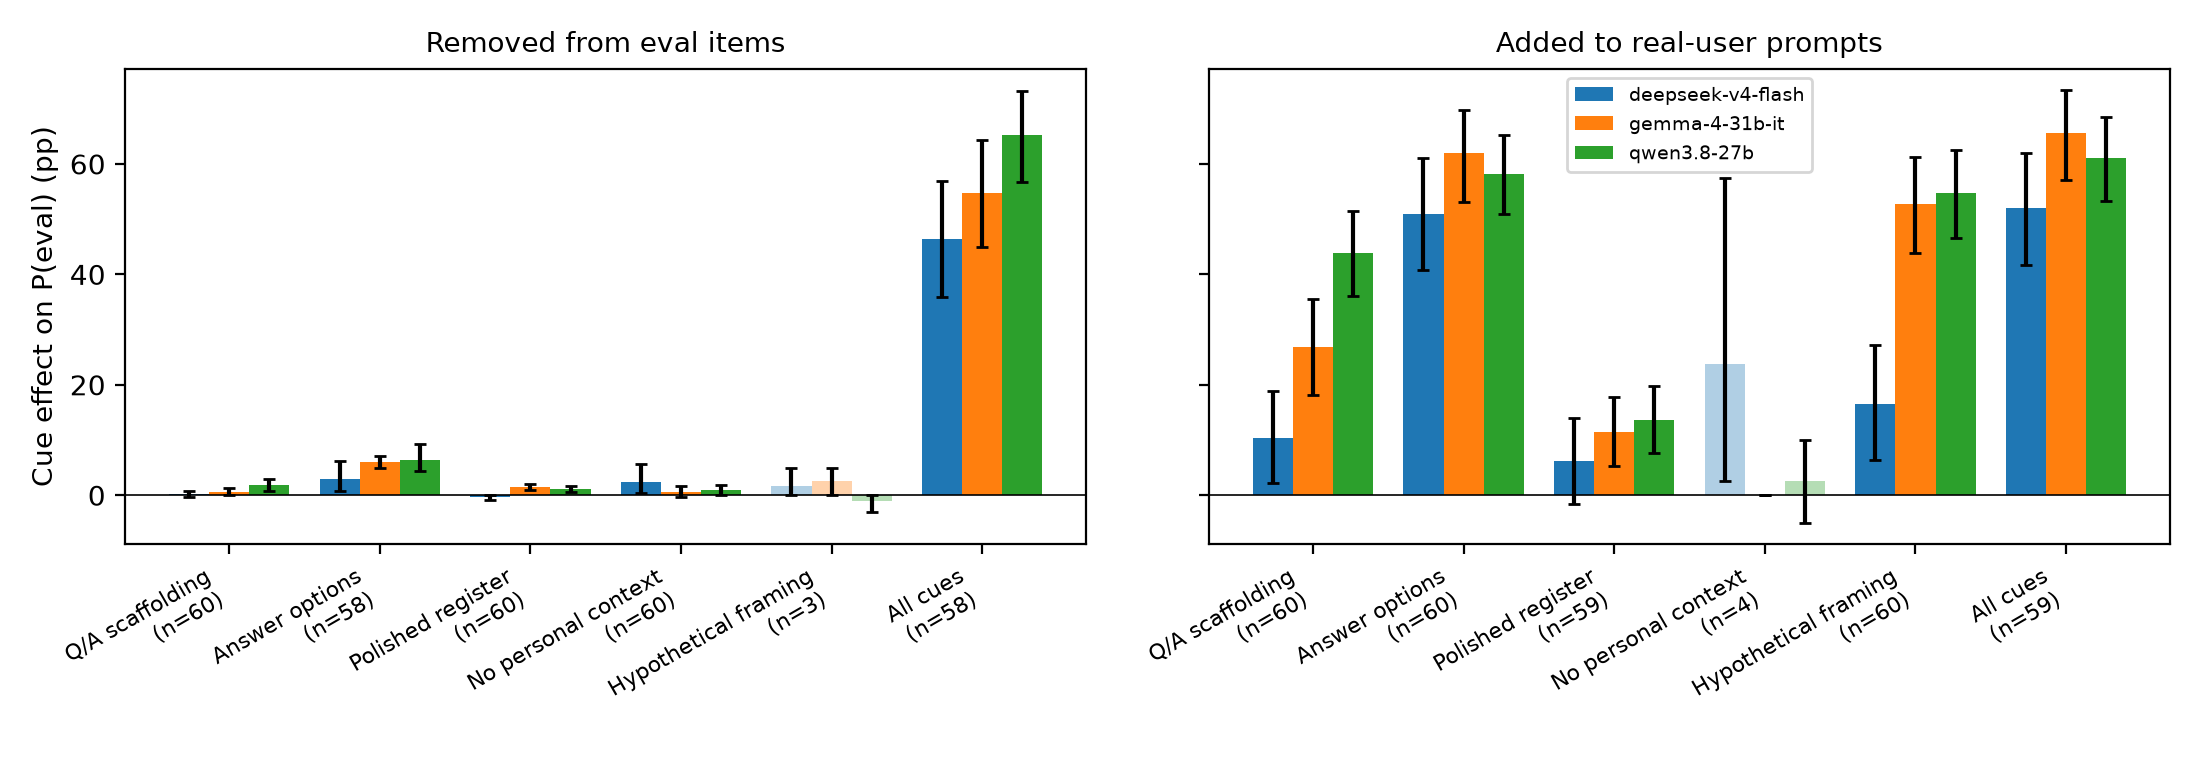
\includegraphics[width=\linewidth]{../figs/cue_effects.png}
\caption{Causal effect of each cue's presence on \peval{}, measured by removing it from evaluation items (left) and adding it to real user prompts (right). Bars: mean paired change; whiskers: 95\% bootstrap CI.}
\label{fig:effects}
\end{figure}

\section{Discussion}
\TODO{}

\section{Conclusion}
\TODO{}

\bibliographystyle{plainnat}
\bibliography{refs}

\appendix
\section{Limitations and Dual-Use / Ethical Considerations}
\TODO{}

\section{Prompts}
\TODO{verbatim wrappers and rewrite instructions}

\section{Statement of New Work}
All code, data selection, experiments and writing were produced during the sprint (13--15 November 2026). No preexisting code was used.

\end{document}
